\begin{figure}[t]
\vspace{-18pt}
\begin{singlespace}

~~
\begin{minipage}{0.46in}
{\centering
\psfig{figure=pipeline.eps,width=0.46in} \\
}
\end{minipage} 
~
\begin{minipage}{1.3in}
{\centering
\psfig{figure=splitjoin.eps,width=1.3in} \\
}
\end{minipage}
~
\begin{minipage}{1.02in}
{\centering
\psfig{figure=feedback.eps,width=1.02in} \\
}
\end{minipage}
~~~~~~~~~
\begin{minipage}{3in}
\vspace{36pt}
\psfig{figure=iir-pipeline.eps, width=2.33in}
~~~~
\raisebox{12pt}{\psfig{figure=iir-pipeline2.eps, width=0.46in}}
\end{minipage}
\\ ~ \\ {\protect\small (a) A pipeline. ~~(b) A splitjoin. ~~(c) A feedbackloop.}

\begin{minipage}{3.5in}
\caption{Stream structures supported by StreamIt.
\protect\label{fig:structures}}
\end{minipage}
\begin{minipage}{3in}
\caption{Example pipeline with IIR filter.\protect\label{fig:iir-pipeline}}
\end{minipage}
\vspace{3pt}
\hrule
\vspace{3pt}

\hfill
\begin{minipage}{2.2in}
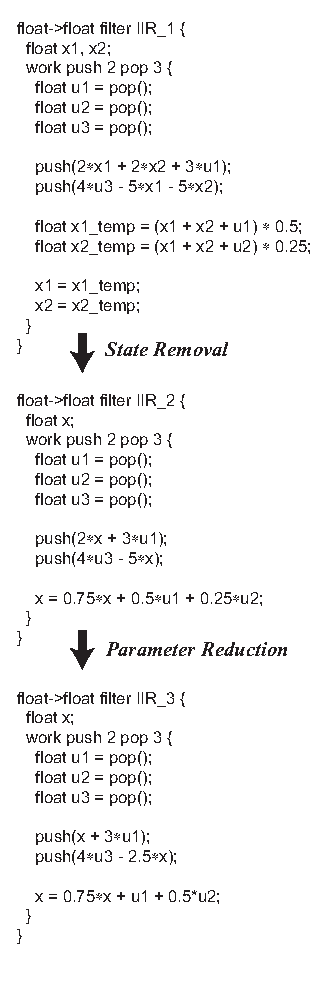
\epsfig{file=statespace-example.eps, width=2.05in}
\end{minipage}
~~~~
\raisebox{10pt}{
\begin{minipage}{3.5in}
Number of multiplications: 8 \\
Number of additions: 8 \\
State space representation:
\begin{eqnarray*}
\small
\vec{\mathbf{y}} & = & \left [ \begin{array} {cc} 2 & 2 \\ -5 & -5
\end{array} \right ] \vec{\mathbf{x}} + \left [ \begin{array} {ccc} 3 & 0 & 0 \\ 0 & 0 & 4 \end{array} \right
 ] \vec{\mathbf{u}} \\
\vec{\dot{\mathbf{x}}} & = & \left [ \begin{array} {cc} 0.5 & 0.5 \\ 0.25
& 0.25 \end{array} \right ] \vec{\mathbf{x}} + \left [ \begin{array} {ccc} 0.5 & 0 & 0 \\
0 & 0.25 & 0 \end{array} \right ] \vec{\mathbf{u}}
\end{eqnarray*}
\vspace{9pt} ~ \\
\hrule
\vspace{12pt} ~ \\
Number of multiplications: 7 \\
Number of additions: 4 \\
State space representation:
\begin{eqnarray*}
\small
\vec{\mathbf{y}} & = & \left [ \begin{array} {cc} 2 \\ -5
\end{array} \right ] \vec{\mathbf{x}} + \left [ \begin{array} {ccc} 3 & 0 & 0 \\ 0 & 0 & 4 \end{array} \right
 ] \vec{\mathbf{u}} \\
\vec{\dot{\mathbf{x}}} & = & \left [ \begin{array} {cc} 0.75
\end{array} \right ] \vec{\mathbf{x}} + \left [ \begin{array} {ccc} 0.5 & 0.25 & 0 \end{array} \right ] \vec{\mathbf{u}}
\end{eqnarray*}
\vspace{-3pt} ~ \\
\hrule
\vspace{12pt} ~ \\
Number of multiplications: 6 \\
Number of additions: 4 \\
State space representation:
\begin{eqnarray*}
\small
\vec{\mathbf{y}} & = & \left [ \begin{array} {cc} 0.5 \\ -1.25
\end{array} \right ] \vec{\mathbf{x}} + \left [ \begin{array} {ccc} 3 & 0 & 0 \\ 0 & 0 & 4 \end{array} \right
 ] \vec{\mathbf{u}} \\
\vec{\dot{\mathbf{x}}} & = & \left [ \begin{array} {cc} 0.75
\end{array} \right ] \vec{\mathbf{x}} + \left [ \begin{array} {ccc} 2 & 1 & 0 \end{array} \right ] \vec{\mathbf{u}}
\end{eqnarray*}
\end{minipage}}
\end{singlespace}
\begin{center}
\vspace{-24pt}

\caption{Example optimization of an IIR filter using linear state
space analysis.  The top segment shows the original code.  The middle
segment depicts the action of state removal, in which the quantity
$x_1 + x_2$ is replaced by a single variable $x$.  The bottom segment
illustrates minimal parameterization, in which the coefficients are
refactored so as to eliminate a multiplication (the coefficient of
$u_2$ becomes 1.)\protect\label{fig:opt-seq}}
\end{center}
\vspace{-12pt}
\end{figure}
